\documentclass[UTF8,a4paper,8pt]{ctexart} 

\usepackage{graphicx}%学习插入图
\usepackage{verbatim}%学习注释多行
\usepackage{booktabs}%表格
\usepackage{geometry}%图片
 \usepackage{amsmath} 
 \usepackage{amssymb}
 
%设置文章宽度
\geometry{textwidth=18cm}
%设置页面布局
\pagestyle{plain}
\author{郑华}
\title{OpenCV 函数简介}

 %正文排版开始
 \begin{document} 
 	\maketitle
 		
\section{读取图片}
	\paragraph{1.imgread}Mat img=imread("D:$ \verb|\\|$美丽姐$ \verb|\\|$Ant$ \verb|\\|$image-0000001.bmp");  
	\paragraph{2.cvLoadImage}从文件中读取图像   const char *pstrImageName = "D:$ \verb|\\|$美丽姐$ \verb|\\|$Ant$ \verb|\\|$image-0000001.bmp";\\
	IplImage *pImage = cvLoadImage(pstrImageName, CV\_LOAD\_IMAGE\_UNCHANGED);  
	
	
\section{显示窗口}
	\paragraph{1.imshow}cvNamedWindow("游戏原画");  \\
	// 在窗口中显示游戏原画  
	imshow("游戏原画",img);  
	\paragraph{2.cvShowImage}	 cvNamedWindow(pstrWindowsTitle, CV\_WINDOW\_AUTOSIZE);  \\
	//在指定窗口中显示图像  
	cvShowImage(pstrWindowsTitle, pImage); 
	
	
	
\section{基本数据结构} 
    \paragraph{1.cvPoint系列}
    表示图像中的点, cvPoint:
    \begin{figure}[h] 	
    	\centering
    	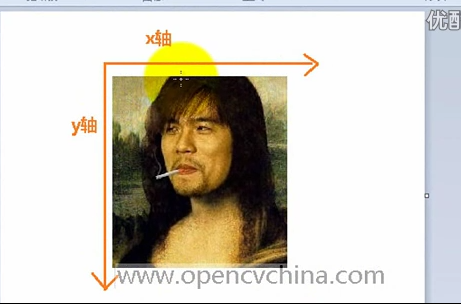
\includegraphics[width=6cm,clip]{point_xy.png} 	
    	\caption{坐标图}	
    	\label{fig:myphoto} 
    \end{figure} 
    cvPoint2D32f : 二维空间中的点
    cvPoint3D32f : 三维空间中的点
	\paragraph{2.cvSize系列}
	表示图像的尺寸,CvSize2D32f 如果想用浮点型; \\
	一个宽度,一个高度。
    \paragraph{3.cvRect}
     矩形框  x,y,width,height
    
    \begin{figure}[h] 	
    	\centering
    	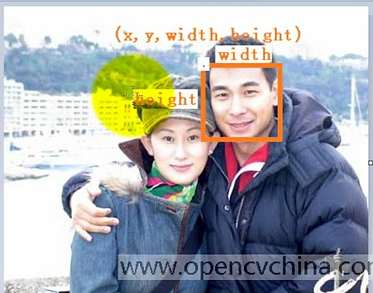
\includegraphics[width=6cm,clip]{cvRect.png} 	
    	\caption{坐标图}	
    	\label{fig:myphoto}
    \end{figure} 
    
    \paragraph{4.cvScalar}
    包含4个double型数据,可以用来表示 B通道,G通道,R通道,Alpha透明度.
    
    构造函数3个 :\\
    cvScalar,cvRealScalar,cvScalarAll
    
    CvScalar s = cvScalar(double B\_Channle, double G\_Channle, double R\_Channle, double Alpha);
    
    // Example: 
    
    CvScalar s = cvScalar(20.0);
    
    s.val[0]=20.0;
    
    \paragraph{5.cvRectangle} 
       cvRectangle(\newline
        myImg,\newline
        cvPoint(5,20),利用构造函数构造一个实例,而免去声明的过程\\
        cvPoint(20,30),\newline
        cvScalar(255,255,255)\newline
      );在(5,10)和(20,30)之间画一个白色矩形
      
    \paragraph{6.cvArr} 
    
    
    \paragraph{7.cvMat 矩阵维度和通道}
    1.创建 矩阵并初始化
    
    cvMat mat;
    
    float data[18] = \{30,60,40,60,50,40,    67,88,55,33,22,97,   59,69,32,46,25,45\};三行六列
    
    cvInitMatHeader(\&mat,      3,     6,CV\_32FC1,data); 
    
    cvInitMatHeader(矩阵变量,行数,列数,数据类型(位数、类型、通道数),数据);
    
    黑白图像
        \begin{figure}[h] 	
        	\centering
        	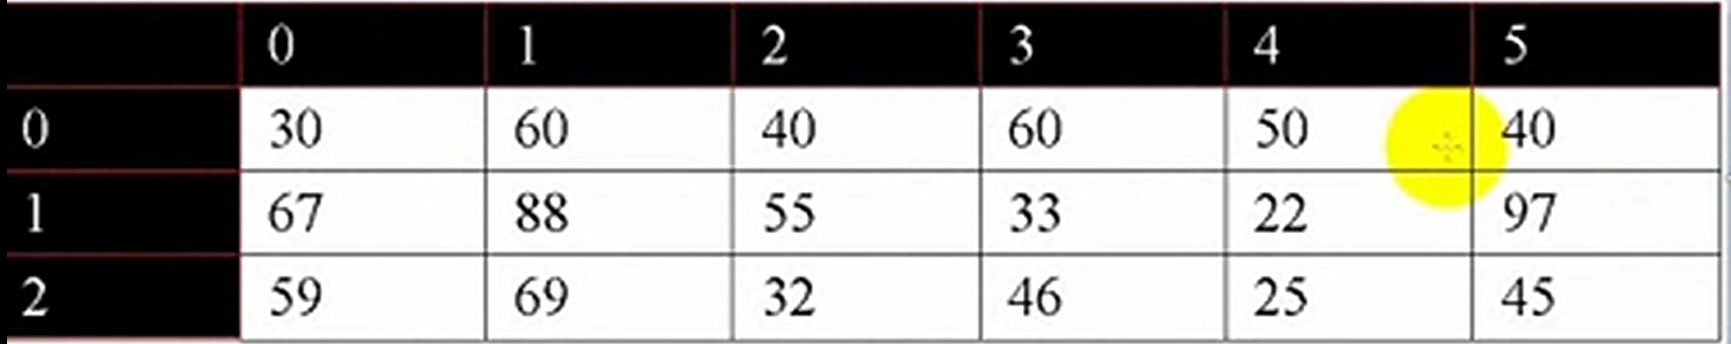
\includegraphics[width=6cm,clip]{singleChannle.png} 	
        	\caption{单通道 存储结果}	
        	\label{fig:myphoto}
        \end{figure} 
        
                cvInitMatHeader(\&mat,      3,     6/2,CV\_32FC2,data); 
                
            灰度图像
            \begin{figure}[h] 	
            	\centering
            	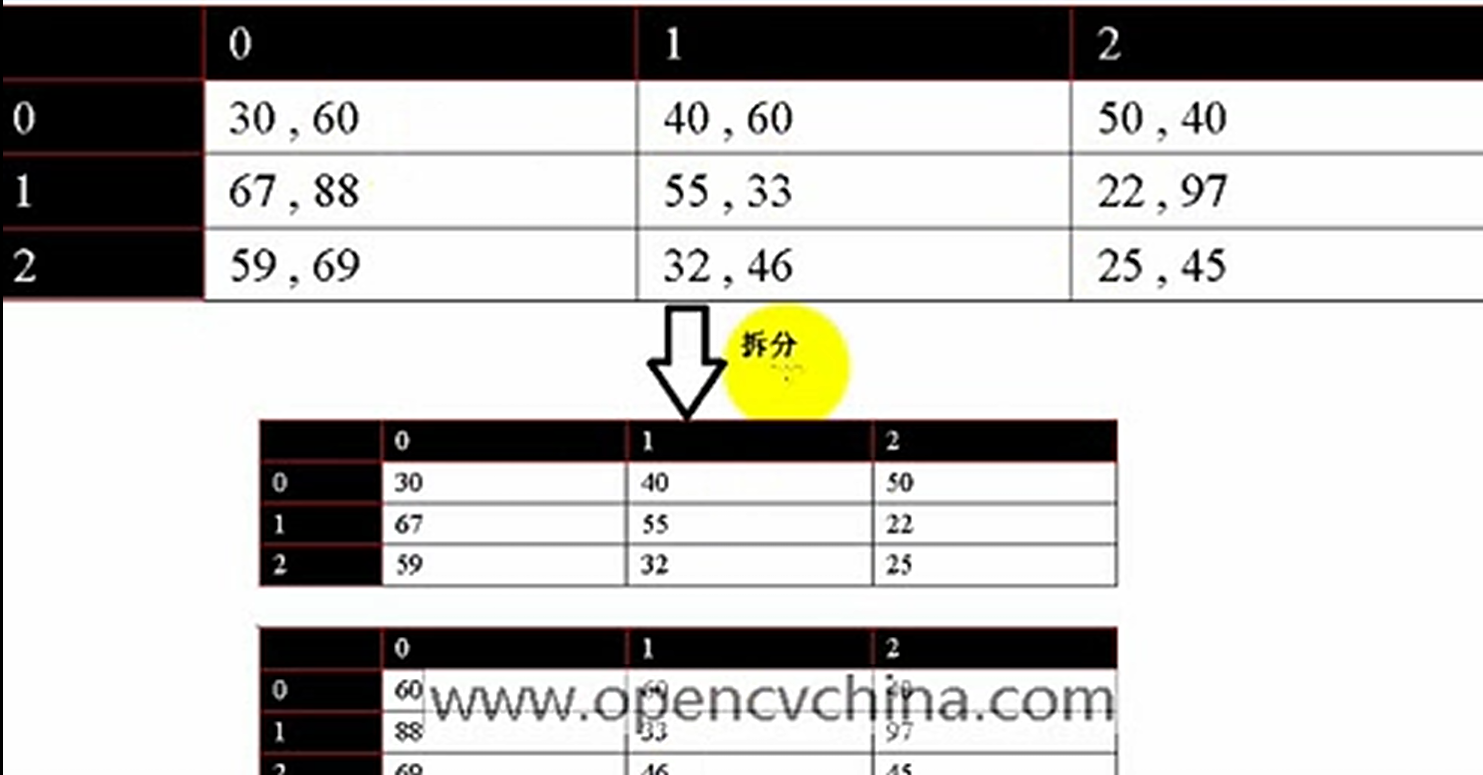
\includegraphics[width=6cm,clip]{doubleChannle.png} 	
            	\caption{双通道 存储结果}	
            	\label{fig:myphoto}
            \end{figure}  
            
             cvInitMatHeader(\&mat,      3,     6/3,CV\_32FC3,data); 
             
            彩色图像
             \begin{figure}[h] 	
             	\centering
             	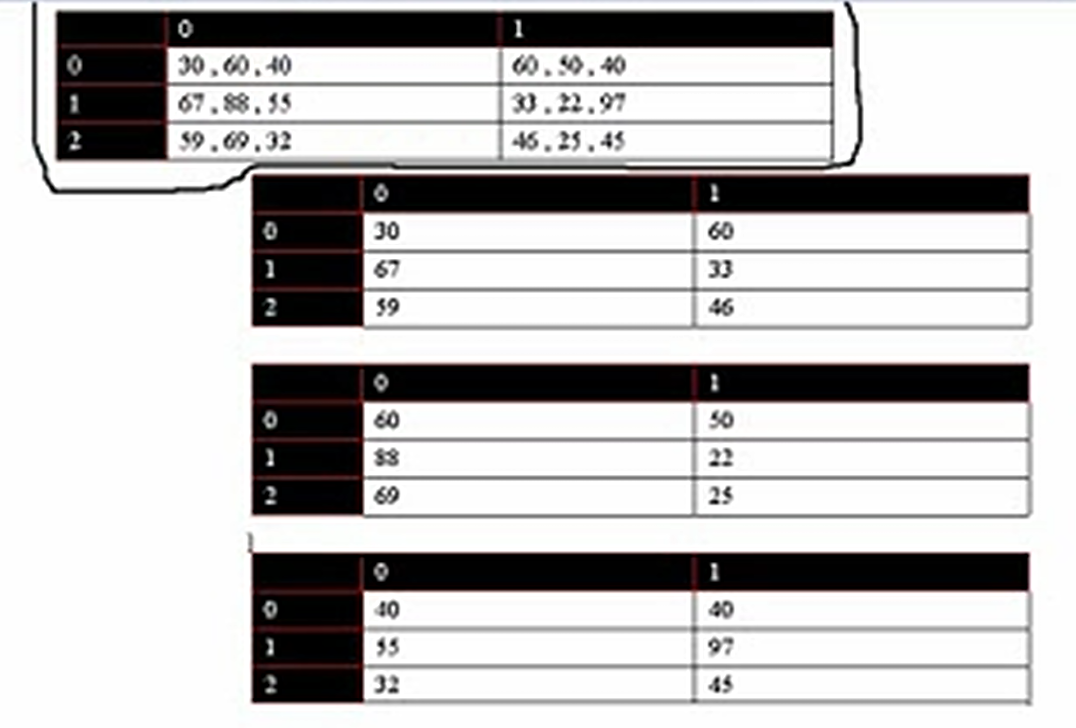
\includegraphics[width=6cm,clip]{threeChannle.png} 	
             	\caption{三通道 存储结果}	
             	\label{fig:myphoto}
             \end{figure}  
    2.相关函数
    
    格式:double cvGetReal2D( const CvArr* arr, int idx\_row, int idx\_column );
    
    作用:返回单通道数组的指定元素
    
    
    3.通道
    
    通道的个数就是说一个元素上存储几个数。 如2
    
    多通道可以分解成单通道。
    
    
    4.维度:就是几维空间的维度,比如3维空间的话就得3个坐标表示一个点(x,y,z)
    
     \paragraph{8.cvMat 矩阵数据访问}
     
     mat.data.ptr + y*mat.step;
     
     mat.step 就是 一行数据的字节数;
     
     \paragraph{9.lpllmage结构}      Width, Height 图像长宽
    
    Depth: usually use IPL\_DEPTH\_*U/S/F (1、8、16、32)每个像素 占用多少个字节数表示,如8u就表示可以有2\^8 = 256种颜色值
    
    nChannals :can be valued 1,2,3,4
    
    origin: only can be valued IPL\_ORIGIN\_TL or IPL\_ORIGIN\_BL
    
    dataOrder: can be valued by IPL\_DATA\_ORDER\_PIXEL or IPL\_DATA\_ORDER\_PLANE
    
    widthStep :临行同列之间的字节数
    
\section{直方图}  
 
 
  \paragraph{1.一维直方图}像素值多少在多少范围,然后对应的峰值也会随之增加,如图
    \begin{figure}[h] 	
    	\centering
    	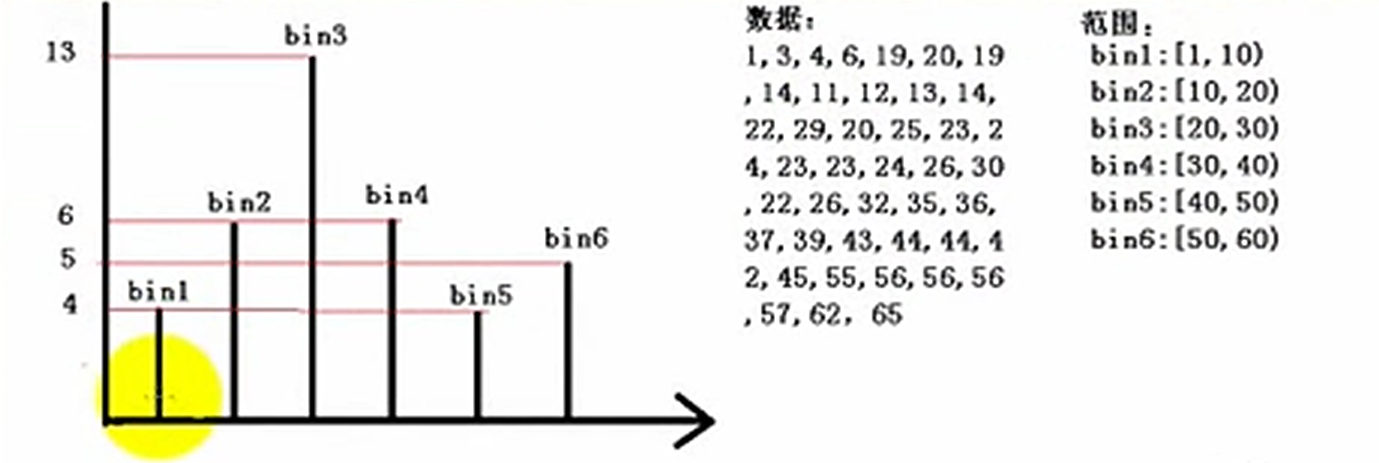
\includegraphics[width=6cm,clip]{histograph.png} 	
    	\caption{一维 单通道 直方图 模型}	
    	\label{fig:myphoto}
    \end{figure}  
   
\end{document} 
		